\section{Sekcja cyfrowa}

\begin{figure}[H]
    \begin{center}
        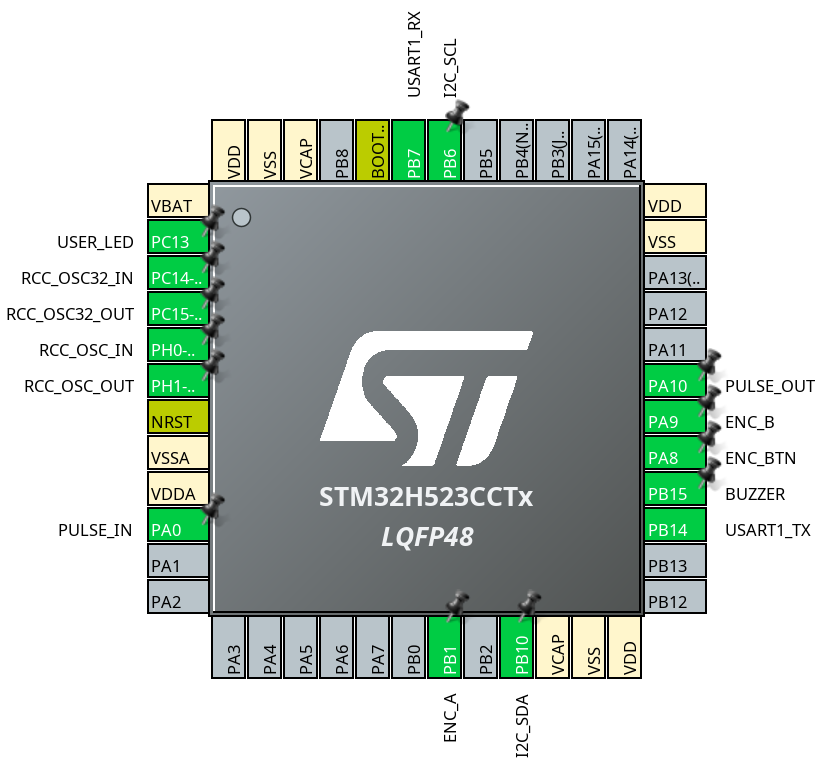
\includegraphics[width=7.5cm]{img/budowa/cube_mx.png}
    \end{center}
    \caption{Cyfrowe przedstawienie układu STM32H523CE wraz z użytymi portami}\label{fig:stm32}
\end{figure}


Część cyfrowa wykrywacza metalu oparta jest o moduł STM32H523CECoreBoard \cite{WeActStudio_STM32H523CoreBoard} zawierający układ \textbf{STM32H523CE}. Ten produkowany przez ST Microelectronics mikrokontroler posiada jeden 32-bitowy rdzeń oparty na architekturze ARM\textregistered{} Cortex-M33\textregistered{} \cite{st_stm32h5_web} \cite{st_stm32h533_ds} o maksymalnym taktowaniu 250Mhz oraz m.in wykorzystane w projekcie układy peryferyjne:

\subsection{Liczniki sprzętowe}
\label{subsec:timery}
Wykorzystywane są dwa 16-bitowe liczniki sprzętowe napędzane za pomocą zegara \textit{APB2} skonfigurowanego na taktowanie z częstotliwością $F_{timer}=250Mhz$.

Konfiguracja oraz interakcja z licznikami w rodzinie układów STM32 odbywa się za pomocą rejestrów:
\begin{itemize}
    \item PSC (Dzielnik, ang. \textit{Prescaler}) - dzieli częstotliwość wejściową $F_{timer}$
    \item ARR (Rejestr Automatycznego Przeładowania, ang. \textit{Auto Reload Register}) - określa długość całego cyklu, po przeładowaniu następuje reset licznika
    \item CCR (Rejestr Przechwytywania i Przeładowania, ang. \textit{Capture/Compare Register}) - w trybie PWM określa moment przełączenia sygnału
    \item CNT (Licznik, ang. \textit{Counter}) - przechowuje aktualną liczbę tyknięć licznika
\end{itemize}

Częstotliwość przepełnienia licznika sprzętowego można wyznaczyć za pomocą poniższego równania: 

\begin{equation}
    F_{output}=\frac{F_{timer}}{(PSC+1)(ARR+1)}
    \label{eq:timer_f}
\end{equation}


Licznik \textit{TIM1} pełni funkcję generatora sygnału \textit{PULSE\_OUT} za pomocą trybu sprzętowego trybu modulacji szerokości impulsów.
Pozwala on na konfigurację częstotliwości oraz wypełnienia sygnału przez mikrokontroler. Jeżeli wartość rejestru \textit{CNT} jest mniejsza od \textit{CCR}, wystawiany jest sygnał +3,3V na pin 1 (PULSE\_OUT) układu, powodując otwarcie tranzystora MOSFET. Następnie w pożądanym momencie sygnał wyjściowy jest wygaszony, co pozwala na dynamiczną konfigurację długości impulsu wysyłanego do cewki.

Drugi licznik \textit{TIM12} wykorzystany jest do generowania sygnału PWM o wypełnieniu 50\% i dynamicznie wyznaczanej częstotliwości do brzęczyka wskazującego o wykryciu anomalii w przetworzonym sygnale \textit{SIGNAL\_OUT}.
Dynamiczna rekonfiguracja rejestrów licznika pozwala na uzyskanie tonu o zadanej częstotliwości. 
Wzór na wartość rejestru ARR można wyznaczyć przekształcając wzór \ref{eq:timer_f}:

\begin{equation}
    ARR = \frac{F_{timer}}{(PSC+1) \cdot f_{target}} - 1
    \label{eq:buzzer_arr}
\end{equation}

W celu uzyskania wypełnienia 50\% należy ustawić rejestr \textit{CCR} na połowę wartości rejestru \textit{ARR}:

\begin{equation}
    CCR = \frac{ARR}{2}
    \label{eq:buzzer_ccr}
\end{equation}

\subsection{Konwerter cyfrowo-analogowy}

ADC napędzany jest sygnałem zegarowym \textit{HCLK} o częstotliwości $F_{ADC}=250Mhz$, z preskalerem o wartości $4$, co daje końcową częstotliwość podukładu wynoszącą $62,5Mhz$.
Maksymalna rozdzielczość pomiaru wynosi 12 bitów, co daje dokładność na poziomie $0,8 mV$.

\begin{equation}
R= \frac{Vref}{2^N - 1} =\frac{3,3V}{4095}\approx 0,8mV
\end{equation}

gdzie $V_{ref}$  to napięcie referencyjne (tutaj $V_{in}=3,3V$), $N$ = liczba bitów

W celu osiągnięcia jak największego zasięgu wykrywacza wymagana jest jednocześnie jak największa dokładność układu ADC oraz jego szybkość działania. Dla trybu 12-bitowego każdy pomiar zajmuje $C_{sample}=15$ cykli zegarowych dających teorytyczny limit przy ustalonym wcześniej taktowaniu zegara ADC wynoszący $4,16 MSPS$ (milionów próbek na sekundę, ang. \textit{Mega Sample Per Second}), co daje jedną próbkę napięcia co $~0,24\mu s$.

\begin{equation}
    SPS = \frac{F_{ADC}}{C_{sample}}=\frac{62,5\cdot10^6}{15}\approx{4,16\cdot10^6}\frac{S}{s}
\end{equation}

Dla maksymalnego odciążenia mikrokontrolera wykorzystany został tryb DMA (bezpośredni dostęp do pamięci, ang. \textit{Direct Memory Access}) z wyłączonym generowaniem przerwań sprzętowych. Każda nowa próbka napięcia wykonana przez konwerter analogowo-cyfrowy zapisywana jest przez układ peryferyjny GPDMA1 do cyklicznego buforu znajdującym się pamięci SRAM wskazanym podczas konfiguracji bez dodatkowego udziału rdzenia Cortex-M33.

\begin{figure}[H]
    \begin{center}
        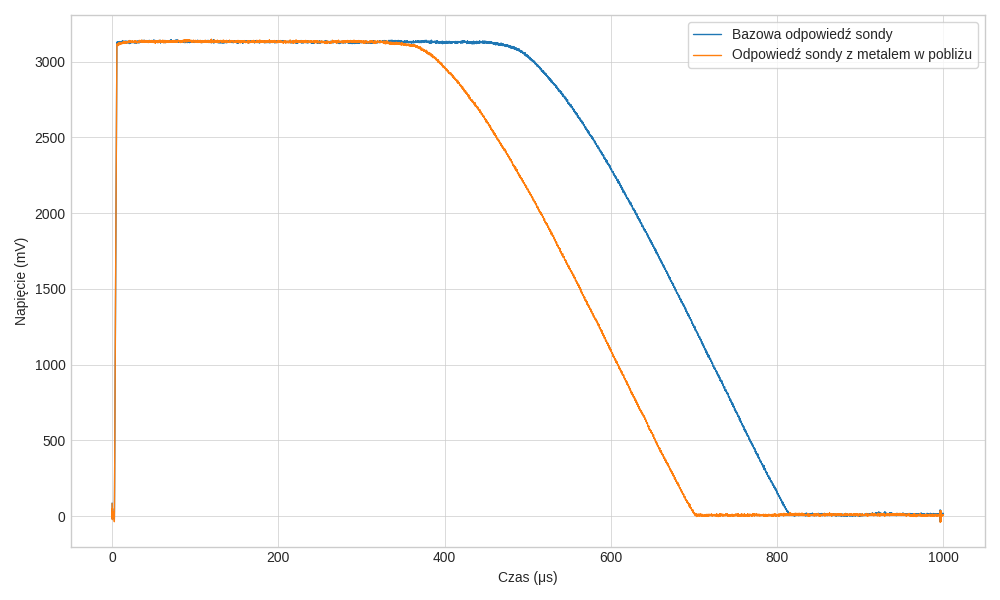
\includegraphics[width=0.95\textwidth]{img/budowa/pulse_out.png}
    \end{center}
    \caption{Wykres odpowiedzi sondy \textit{PULSE\_OUT}}\label{fig:pulse_out}
\end{figure}

W celu dokładnego wyznaczenia trwania nasyconej odpowiedzi sondy wykorzystywany jest wbudowany w ADC sprzętowy komparator okienkowy (Analog Watchdog, AWD). To peryferium konwertera analogowo-cyfrowego pozwala na wyznaczenie zakresu wartości próbek, którego opuszczenie wywoła przerwanie mikrokontrolera. W prototypie moduł ten skonfigurowany jest na wykrywanie momentu przekroczenia przez sygnał wartości dolnej granicy wynoszącej 3000. Górna granica okna wynosi 4095, czyli maksymalną wartość próbki przy rozdzielczości 12-bitów, efektywnie eliminując możliwość wywołania przerwania.


Algorytm napędzający prototyp wykrywacza metali wykorzystuje komparator okienkowy w celu wykrywania anomalii czasu trwania odpowiedzi sondy.
Jak można zauważyć na wykresie \ref{fig:pulse_out}, podczas przybliżenia metalowego obiektu zmienia się charakterystyka sygnału \textit{SIGNAL\_OUT}.
Wykorzystanie sprzętowego rozwiązania pozwala na dokładne wyznaczenie momentu przekroczenia granicy 2,01V ($\frac{2500}{4095}\cdot 3,3V$). Kod przerwania wywołanego przez AWD zapisuje w pamięci mikrokontrolera aktualną wartość licznika \textit{TIM1}, co pozwala dokładnie odtworzyć względny czas wywołania przerwania po wyłączeniu sygnału \textit{PULSE\_OUT}. Przechwycona wartość mnożona jest przez czas pomiędzy inkrementacją licznika.

